\documentclass{scrartcl}% siehe <http://www.komascript.de>
\usepackage{selinput}% Eingabecodierung automatisch ermitteln …
\usepackage{hyperref}
\SelectInputMappings{% … siehe <http://ctan.org/pkg/selinput>
  adieresis={ä},
  germandbls={ß},
}
\usepackage{graphicx}
\usepackage[ngerman]{babel}% Das Beispieldokument ist in Deutsch,
                % daher wird mit Hilfe des babel-Pakets
                % über Option ngerman auf deutsche Begriffe
                % und gleichzeitig Trennmuster nach den
                % aktuellen Rechtschreiberegeln umgeschaltet.
                % Alternativen und weitere Sprachen sind
                % verfügbar (siehe <http://ctan.org/pkg/babel>).
                
\setlength{\parskip}{0.2cm}  % 2mm Abstand zwischen zwei Absätzen
\setlength{\parindent}{0mm}  % Absätze nicht einziehen
\usepackage[backend=biber,
isbn=false,                     % ISBN nicht anzeigen, gleiches geht mit nahezu allen anderen Feldern
sortlocale=de_DE,               % Sortierung der Einträge für Deutsch
%sortlocale=en_US,              % Sortierung der Einträge für Englisch
autocite=inline,                % regelt Aussehen für \autocite (inline=\parancite)
hyperref=true,                  % Hyperlinks für Ziate
style=ieee                     % Zitate als Zahlen [1]
%style=alphabetic               % Zitate als Kürzel und Jahr [Ein05]
%style=authoryear                % Zitate Author und Jahr [Einstein (1905)]
]{biblatex} 
\addbibresource{literatur.bib}
\setlength{\bibitemsep}{1em}     % Abstand zwischen den Literaturangaben
\setlength{\bibhang}{2em}        % Einzug nach jeweils erster Zeile

% Trennung von URLs im Literaturverzeichnis (große Werte [> 10000] verhindern die Trennung)
\defcounter{biburlnumpenalty}{10} % Strafe für Trennung in URL nach Zahl
\defcounter{biburlucpenalty}{500}  % Strafe für Trennung in URL nach Großbuchstaben
\defcounter{biburllcpenalty}{500}  % Strafe für Trennung in URL nach Kleinbuchstaben

\begin{document}
% ----------------------------------------------------------------------------
% Titel (erst nach \begin{document}, damit babel bereits voll aktiv ist:
\titlehead{AMR}% optional
\subject{Projektbericht AMR}% optional
\title{Kartierung der WLAN Signalstärke}% obligatorisch
%\subtitle{Untertitel}% optional
\author{Florian Zirker, Lukas Arnecke}% obligatorisch
%\date{z.\,B. der Abgabetermin}% sinnvoll
\publishers{Prof. Dr. Thomas Ihme}% optional
\maketitle% verwendet die zuvor gemachte Angaben zur Gestaltung eines Titels
% ----------------------------------------------------------------------------
% Inhaltsverzeichnis:
\tableofcontents
% ----------------------------------------------------------------------------
% Gliederung und Text:

\section{Einleitung}
\textbf{Muss noch überarbeitet werden}

Eine moderne Hochschule ist auf eine funktionierende Netzwerkinfrastruktur angewiesen. Dazu gehört auch eine möglichst vollständige WLAN-Abdeckung, damit sowohl Studenten als auch Dozenten und Mitarbeiter ihre jeweiligen Aufgaben erfüllen können auch wenn sie sich nicht an einem fest installierten Rechner befinden.

Um genau diese WLAN-Abdeckung zu prüfen und eventuelle Lücken konkret aufzeigen zu können gab es im Rahmen der Vorlesung \textit{Autonome Mobile Roboter (AMR)} das Projekt, die Signalstärke mithilfe eines Roboters flächendeckend aufzeichnen zu können.

\textbf{Ab hier weiter!}

\newpage
\section{Grundlagen}
\subsection{Pioneer 3-DX Roboter}
Der mobile Forschungsroboter Pioneer 3-DX ist eine Roboterplattform, die für fast alle Anwendungen modifizierbar ist. Er besteht im Grunde nur aus einem Motor, Reifen und einer Plattform, durch die benötigte Module angebracht werden können \cite{pioneer}. Die Steuerungseinheit ist so gebaut, dass sie über das \textit{Robot Operating System} (ROS) angesprochen werden kann.

\begin{figure}[h]
	\centering
	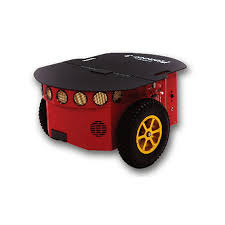
\includegraphics{bilder/pioneerRoh.jpg}
	\caption{Pioneer 3-DX Roboter ohne Aufbauten \cite{pioneer}}
	\label{pioneerRoh}
\end{figure}

Auf der Plattform ist ein Laser, ein Wlan-Modul und eine Rechner aufgebaut, mit deren Hilfe die Kartierung durchgeführt wird. Auf dem Rechner läuft Ubuntu 18.04 LTS, auf welchem wiederum ROS in der Version Melodic installiert ist.

\subsection{Robot Operating System}
\textit{ROS} ist ein Open Source Framework, welches speziell für auf die Nutzung für autonome Systeme entwickelt wurde. Die Idee von ROS ist die Bereitstellung von wiederverwendbaren Modulen, von denen jedes eine eigene Aufgabe erfüllen kann und die beliebig kombiniert werden können \cite{rosIntro}.

Für ein möglichst einfaches Management liefert ROS eine eigene Paketverwaltung, mit der die benötigten Pakete nachinstalliert werden können. Ein Paket enthält unter Anderem den Quellcode und Launchfiles für die \textit{Nodes}, in denen die Berechnungen stattfinden \cite{rosIntro2}. Jeder Node ist für andere Berechnungen zuständig, so gibt es einen Node für die Koordinatentransformationen zwischen den einzelnen Bauteilen des Roboters, einen für den Laserscanner, einen für die Berechnung der WLAN-Signalstärke und einen für die Ansteuerung des Motors.

Die Kommunikation zwischen Nodes, wie in  läuft über ein Publisher/Subscriber Prinzip, das bedeutet, dass ein Node, wie in Abbildung \ref{concept} dargestellt, definierte Informationen über einen \textit{Topic} veröffentlicht. Diese Topics können wiederum von anderen Nodes abgegriffen und weiter verarbeitet werden. Die enthaltenen Informationen werden über \textit{Messages} ausgetauscht, wodurch sowohl die Struktur als auch der Inhalt klar definiert sind. Alle Nodes müssen sich bei dem \textit{Master}, dem Namens- und Registrierungsservice innerhalb der ROS Umgebung, registrieren, um sich gegenseitig zu finden und dann auch Daten austauschen zu können \cite{rosKonzept}.

\begin{figure}
	\centering
	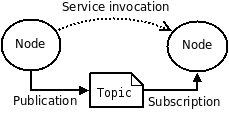
\includegraphics{bilder/ROS_concepts.png}
	\caption{Schematischer Aufbau der Kommunikation \cite{rosKonzept}}
	\label{concept}
\end{figure}

\subsection{Kartierung}
Für die Kartierung bietet ROS das Package \textit{gmapping}, wenn die Karte mithilfe eines Lasermoduls erstellt werden soll. Dieses Package bietet die Funktionalität, um eine laserbasierte Karte mithilfe des Systems \textit{Simultaneous Localization and Mapping} (SLAM) zu erstellen. Hierbei wird eine 2D Karte aus der Kombination von den Laserdaten und der vermuteten eigenen Position erstellt. Die Daten über die eigene Position kommen aus den Odometriedaten, also der vermuteten Bewegungsrichtung und -distanz anhand der Bewegungen der Räder. Der Node \textit{slam\_gmapping} subscriped die Topics \textit{tf} und \textit{scan}, aus denen es dann die Karte berechnet und unter dem Topic map veröffentlicht. \cite{gmap}. Die Abschätzung des Drehwinkels um die eigene Achse durch Odometrie ist vergleichsweise ungenau, weshalb es zu fehlerhaften Karten kommen kann, wenn der Roboter während der Kartierung zu viele Kurven fährt. Der Abgleich mit den Laserdaten wirkt diesem Effekt entgegen, bei einem erneuten Abfahren des Bereiches können entstandene Verschiebungen erkannt und behoben werden.

\subsection{Wireless Local Area Network}
In dieser Sektion wird folgendes erklärt:
\begin{itemize}
	\item WLAN (Funkmodi, Standards, )
	\item Kanäle 2,4 GHz und 5GHz
	\item Messungen
	\item RSSI-Wert
	\item ...
\end{itemize}
% Zuständigkeit: Flo

\newpage
\section{Problemstellung}
% Eventuell können wir hier noch weiter unterscheiden: Inbetriebnahme, Kartierung und WLAN-Messung. Bin mir nicht sicher. FZ
Im Rahmen des Projektes gibt es verschiedene Problemstellungen, welche zwar aufeinander aufbauen, jedoch trotzdem in sich abgeschlossene Vorgaben beinhalten.

\subsection{Inbetriebnahme}
Der Stand des Roboters vor Beginn des Projektes war, dass auf dem aufgebautem Rechner Ubuntu 14.04 LTS installiert war, auf dem wiederum ein Dockersystem lief. ROS lief dann unter Docker, wodurch verschiedene Konfigurationen parallel auf einem Roboter genutzt werden konnten. Da die ROS Version sich mit der Ubuntuversion ändert lief hier entsprechend auch ROS Kinetic.

Ziel ist es, auf eine neuere ROS Version umzusteigen, um auch neu implementierte Funktionen nutzen zu können. Daher muss neben ROS auch Ubuntu neu installiert und in diesem Zuge geprüft werden, ob an dem Ansatz mit Docker festgehalten wird.

\subsection{Kartierung}
Das neu installierte System soll eine Karte aus dem abgefahrenen Gebiet erstellen und diese anzeigen können. Hierbei sollte beachtet werden, dass die Karte sowohl durch manuelles Fahren erstellt werden kann, als auch eine bereits bestehende Karte hinterlegt werden kann, um dann nach dieser eine vorgegebene Strecke abzufahren. Im Hinblick auf das eigentliche Thema, das Kartieren der WLAN Signalstärke, liegt der Schwerpunkt jedoch entsprechend nicht auf der Umgebungskartierung.

\subsection{WLAN-Messung}
Neben der 2D Karte auf dem vorherigen Kapitel soll auch das WLAN kartografiert werden. Hierbei soll die Signalstärke für ein angegebenes Netz synchronisiert auf die aktuelle Position des Roboters aufgezeichnet werden.

Desweiteren soll eine Möglichkeit gefunden werden, die erhobenen Daten als Heatmap auf einer Karte zu visualisieren.

\newpage
\section{Realisierung}
\subsection{Genutzte Tools}
Für das Projekt wurde der Rechner auf dem Roboter komplett neu aufgesetzt. Für ein möglichst modernes System wurde Ubuntu 18.04 LTS installiert, wofür dann ROS in der Version Melodic vorgesehen ist und aus diesem Grund installiert wurde.

Desweiteren 


\subsection{Architektur}
Wir setzen auf ROS. Was wiederum auf dem Betriebsystem sitzt. Wir nutzen das Messaging-System (Publisher/Subscriber). Wir nutzen p2os was wiederum auf ??? nutzt. Wir schreiben unseren eigenen Knoten.

\subsection{Aufgetretene Probleme}
% Wollen wir  wirklich in einem Kapitel erklären was für Probleme wir hatten? Ich denke es macht mehr sinn die einzellnen Schritte genauer zu erklären und dann an der entsprechenden Stelle zu erklären was schwierig war. (Siehe folgende Kapitel)
ROS Melodic ist zwar veröffentlicht und für Ubuntu 18.04 vorgesehen, jedoch sind noch nicht alle Funktionen der Vorgängerversionen implementiert. Das führte dazu, dass manche Aufrufe der Launchscripte manuell umgeschrieben und ROS neu kompiliert werden musste.

Auch war das Extrahieren der Signalstärken erwies sich als Problem.
%Sollte Flo möglichst ausfüllen

\subsection{Inbetriebnahme und Installation}
% Alles veraltet. Vorhergehende Gruppe hat Docker ansazt gewält, nicht mehr lauffähig. Neues Betriebsystem. Neues ROS. Damit einige Probleme: Selbstcompilieren einiger Pakete nötig. 

\subsection{Simultaneous Localization and Mapping}

\subsection{Aufzeichnung der Fahrt}

\subsection{Kartenerstellung aus aufgezeichneter Fahrt}

\subsection{WLAN-Messung}
% Zuständig:Flo

\section{Ergebnisse}
%Was ist raus gekommen. Neue Erkenntnisse, Lösungen, Unsere zwei Karten.

\section{Zusammenfassung}

\newpage
\section{Ausblick}
Die Datenerhebung funktioniert. Der nächste Schritt wäre, mit dem Roboter strukturiert ein Gebiet zu kartieren und eine Flächendeckende Abdeckung zu erstellen. Auch würde eine Lösung, mit der eine Heatmap in RVIZ oder direkt danach überlagert eingeblendet werden kann, die Nachbearbeitung deutlich vereinfachen.


\newpage
% Literaturverzeichnis erzeugen
\begin{flushleft}
	\printbibliography
\end{flushleft}


\end{document}
